\section{Measured computational cost and repeated parameter evaluation}
\subsection{Experimental design and independent baselines}
Numerical correctness and elapsed time are distinct properties. We
therefore benchmark the same PLS estimator at matched $(n,d,\mu)$
and identical candidate penalties, using four implementations:
(i) a deliberately naive dense solver that reconstructs $D_d$,
$Q_d=D_d^\top D_d$, and solves the normal equations at every
candidate; (ii) a denser but fairer baseline that caches $Q_d$ and
repeats its dense solve; (iii) the reusable full-SVD spectral
implementation of \texttt{TrendSmoother}; and (iv) a banded solver
that assembles $Q_d$ directly in its sparse-band storage and uses
a structure-aware linear solver. The last comparison is crucial:
beating dense normal equations does not imply beating specialized
PLS solvers \cite{weinert2007wh,weinert2012fast}.

\paragraph{Banded factorization and benchmark scope.}
For every finite $\lambda\geq0$, the normal-equation matrix
$A_\lambda=I_n+\lambda D_d^\top D_d$ is symmetric positive
definite, since $x^\top A_\lambda x=\|x\|_2^2+
\lambda\|D_dx\|_2^2>0$ for any nonzero $x$.
It has half-bandwidth $d$, so a banded Cholesky factorization
$A_\lambda=L_\lambda L_\lambda^\top$ is a valid
structure-aware solution method. Its factor generally must be
recomputed when $\lambda$ changes, whereas a spectral basis
can be reused across penalties. This is established computational
prior art \cite{weinert2007wh,weinert2012fast}.

Importantly, the \emph{banded} timings in the four-method
tables below come from \texttt{scipy.linalg.solve\_banded},
a general banded linear-system solver in
\texttt{paper/benchmarks/run\_benchmarks.py}; they are
\emph{not} measured Cholesky timings. The separate library
backend \texttt{PreparedPLSSolver(method="cholesky")} in
\texttt{src/trendestimation/solvers.py} instead calls
\texttt{scipy.linalg.cholesky\_banded} followed by
\texttt{scipy.linalg.cho\_solve\_banded} to produce full
fitted trends. Neither its timings nor Weinert's QR or FFT
methods are included in these four-method tables.
We therefore make no measured Cholesky-specific speed
claim from this experiment.

For every case a deterministic Gaussian sequence is generated,
$\mu$ is held at either zero or a fixed nonzero value, and
$\lambda$ spans $10^{-3}$ to $10^3$ on a geometric grid.
The \texttt{quick} experiment varies $n\in\{40,100,180\}$,
$M\in\{1,16,64\}$ with $d=2$ and adds
$d\in\{1,3,5\}$ at $n=100$, $M=24$, together
with a nonzero-$\mu$ case. The \texttt{full} experiment reaches
$n=400$, $M=256$ and additional difference orders.
All results include one-time setup (not only post-SVD solves);
we record medians, extrema, and median absolute deviations over
repeated independent runs. We bound maximum disagreement against
an independent banded solve for \emph{every} tested penalty.
Runs use a declared random seed, source revision, machine
metadata, NumPy/SciPy versions and a stated BLAS-thread limit.
The code and machine-readable outputs are confined to
\texttt{paper/benchmarks/}.

\begin{table}[tbp]
\centering
\caption{Leading arithmetic complexity for $M$ reconstructed
trends of length $n$ and fixed order $d$. Setup is counted
and no exact operation counts or GPU measurements are asserted.}
\label{tab:complexity}
\begin{tabular}{lll}
\toprule
Method & Setup & Repeated full fits \\
\midrule
Fresh dense solves & rebuilt per $\lambda$ & $O(Mn^3)$ \\
Cached dense $Q_d$ & dense penalty matrix & $O(Mn^3)$ \\
Spectral SVD & $O(n^3)$ & $O(Mn^2)$ \\
Direct banded solver & $O(nd^2)$ & $O(Mnd^2)$ \\
\bottomrule
\end{tabular}
\end{table}

\subsection{End-to-end full-fit timing results}
\IfFileExists{benchmarks/results/full_fit_table.tex}{%
\begin{table}[tbp]
\centering
\caption{Host-measured end-to-end median times in milliseconds, including
one-time setup, for $M$ full fitted trends. Every method computes
the same trends for the same $n$, $d=2$ and $\mu=0$; $R$ is the
naive-fresh-dense time divided by the spectral time. Values and the
numerical parity check are generated from the raw CSV files, not
entered manually.}
\label{tab:full-fit-timings}
\begin{tabular}{rrrrrrr}
\toprule
$n$ & $M$ & Fresh & Cached & Spectral & Banded & $R$ \\
\midrule
40 & 1 & 0.029 & 0.027 & 0.204 & 0.123 & 0.14 \\
40 & 64 & 1.388 & 0.739 & 1.302 & 1.032 & 1.07 \\
100 & 1 & 0.075 & 0.073 & 0.801 & 0.281 & 0.09 \\
100 & 64 & 4.589 & 2.642 & 2.013 & 1.532 & 2.28 \\
200 & 1 & 0.471 & 0.350 & 3.580 & 0.535 & 0.13 \\
200 & 64 & 20.984 & 10.348 & 4.982 & 2.017 & 4.21 \\
400 & 1 & 3.192 & 3.217 & 20.165 & 1.103 & 0.16 \\
400 & 64 & 196.554 & 106.894 & 20.885 & 3.188 & 9.41 \\
\bottomrule
\end{tabular}

\end{table}
}{%
\noindent\emph{No host-verified timing table is bundled:
execute \texttt{python paper/benchmarks/run\_all.py}
on the reference computer to generate the CSV measurements and
LaTeX table before submitting this manuscript.}\par
}
The crossover between methods should be evaluated using
\emph{end-to-end} times, including the SVD setup cost, for both
a single smoothing parameter and a repeated-$\lambda$ sweep.
A ratio greater than one denotes a speed advantage over the
naive baseline on the reported machine, not a universal speedup.
In particular, the structured banded baseline can outperform
a reusable SVD for full trend reconstruction.

\subsection{Scalar smoothness and EDF are different workloads}
To evaluate $\operatorname{tr}(H_\lambda)$ repeatedly, the
spectral method needs only $n-d$ positive eigenvalues:
\[
\operatorname{tr}(H_\lambda)
=d+\sum_{j=1}^{n-d}(1+\lambda\delta_j)^{-1}.
\]
This is $O(Mn)$ work \emph{after} spectral setup, not
$O(Mn^2)$ reconstructed trends. An independent second
experiment compares repeated dense computations
of $\operatorname{tr}[(I+\lambda Q_d)^{-1}]$,
a banded solver applied to all $n$ canonical right-hand
sides, and the spectral sum. The experiment checks
algebraic equivalence separately from timed regions.
Even when the spectral trace is the most efficient
\emph{marginal} score after setup, the $O(n^3)$ SVD cost
can still dominate small workloads.

\IfFileExists{benchmarks/results/trace_table.tex}{%
\begin{table}[tbp]
\centering
\caption{Median end-to-end times (milliseconds) to evaluate $M$
effective-degrees-of-freedom traces, including setup. These entries
measure only scalar $\operatorname{tr}(H_\lambda)$ quantities, not
reconstructed trends.}
\label{tab:trace-timings}
\begin{tabular}{rrrrrr}
\toprule
$n$ & $M$ & Fresh & Cached & Spectral & Banded \\
\midrule
40 & 8 & 0.213 & 0.150 & 0.203 & 0.322 \\
100 & 8 & 1.059 & 0.832 & 0.801 & 1.072 \\
100 & 32 & 4.220 & 3.307 & 0.885 & 3.615 \\
180 & 32 & 15.914 & 12.208 & 2.830 & 10.114 \\
250 & 64 & 92.614 & 59.421 & 6.090 & 38.391 \\
\bottomrule
\end{tabular}

\end{table}
}{}
\IfFileExists{benchmarks/results/benchmark_environment.tex}{%
\noindent\textbf{Measurement provenance:} Platform: Windows-10-10.0.26100-SP0; CPU: Intel64 Family 6 Model 183 Stepping 1, GenuineIntel; Logical CPUs: 32; NumPy: 2.4.6; SciPy: 1.17.1; BLAS threads: 1; Repetitions: 7; Preset: full; Revision: local-unrecorded.

\noindent Maximum observed absolute trend disagreement: $4.32e-10$; maximum EDF trace disagreement: $5.48e-12$.

}{%
\noindent\emph{Computer specifications, software versions, repetition
counts and source revision will appear here after the benchmarks
are run and saved on the reference host.}\par
}

\IfFileExists{figures/full_fit_at_M64.pdf}{%
\begin{figure}[tbp]
\centering
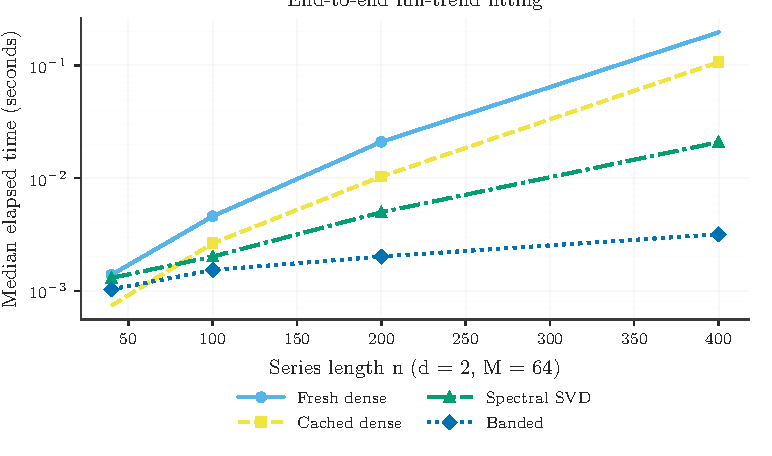
\includegraphics{figures/full_fit_at_M64.pdf}
\caption{End-to-end median times for $M=64$ fitted curves, including setup,
generated on the executing host from the raw CSV files.
These are hardware-specific measurements, not an assumption that
spectral reconstruction is the universally fastest method.}
\label{fig:timing-full}
\end{figure}
}{%
\noindent\emph{The full-fit timing figure is generated after a manually
requested benchmark run with $M=64$.}\par
}

\IfFileExists{figures/trace_at_M32.pdf}{%
\begin{figure}[tbp]
\centering
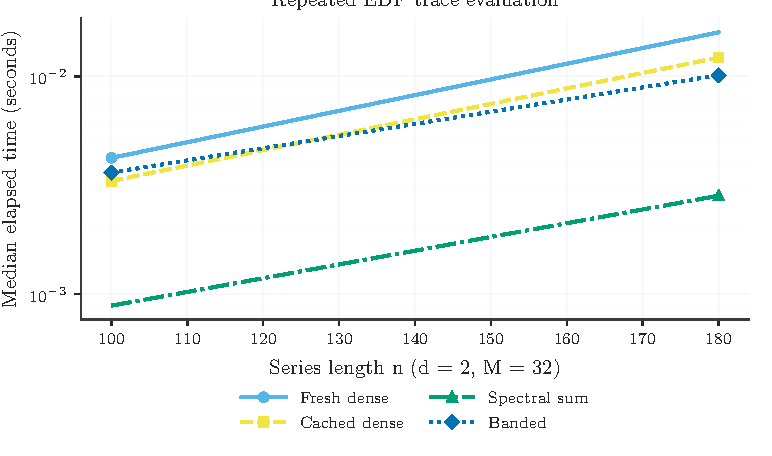
\includegraphics{figures/trace_at_M32.pdf}
\caption{Repeated effective-degrees-of-freedom trace evaluations
($M=32$), including preprocessing. The quantity is scalar
$\operatorname{tr}(H_\lambda)$, not a full trend reconstruction.}
\label{fig:timing-trace}
\end{figure}
}{}

\subsection{Interpreting speed and computational cost}
A timed speed ratio is defined by the two end-to-end
medians, for example
$R_{\rm dense/spectral}
=t_{\rm dense}/t_{\rm spectral}$.
A value above one favors the spectral approach for the
tested workload, not for arbitrary data lengths or
hardware. CPU time, wall time, arithmetic complexity
and energy consumption are different quantities.
CPU numerical libraries already use optimized native
linear algebra, but this experiment does not establish
GPU execution or electricity use. An explicit device
and power measurement would be necessary to make
either claim. Results are intentionally generated
only through a manual command, so the manuscript
does not inadvertently contain timings from a
different machine presented as those of its authors.
